% !TeX spellcheck = en_US
\documentclass[aspectratio=169]{../latex_main/tntbeamer}  % you can pass all options of the beamer class, e.g., 'handout' or 'aspectratio=43'
\usepackage{dsfont}
\usepackage{bm}
\usepackage[english]{babel}
\usepackage[T1]{fontenc}
%\usepackage[utf8]{inputenc}
\usepackage{graphicx}
\graphicspath{ {./figures/} }
\usepackage{algorithm}
\usepackage[ruled,vlined,algo2e,linesnumbered]{algorithm2e}
\usepackage{hyperref}
\usepackage{booktabs}
\usepackage{mathtools}

\usepackage{amsmath,amssymb}
\usepackage{latexsym}

\DeclareMathOperator*{\argmax}{arg\,max}
\DeclareMathOperator*{\argmin}{arg\,min}

\usepackage{pgfplots}
\pgfplotsset{compat=1.16}
\usepackage{tikz}
\usetikzlibrary{trees} 
\usetikzlibrary{shapes.geometric}
\usetikzlibrary{positioning,shapes,shadows,arrows,calc,mindmap}
\usetikzlibrary{positioning,fadings,through}
\usetikzlibrary{decorations.pathreplacing}
\usetikzlibrary{intersections}
\pgfdeclarelayer{background}
\pgfdeclarelayer{foreground}
\pgfsetlayers{background,main,foreground}
\tikzstyle{activity}=[rectangle, draw=black, rounded corners, text centered, text width=8em]
\tikzstyle{data}=[rectangle, draw=black, text centered, text width=8em]
\tikzstyle{myarrow}=[->, thick, draw=black]

% Define the layers to draw the diagram
\pgfdeclarelayer{background}
\pgfdeclarelayer{foreground}
\pgfsetlayers{background,main,foreground}

\newcommand{\comment}[1]{
	\noindent
	%\vspace{0.25cm}
	{\color{red}{\textbf{TODO:} #1}}
	%\vspace{0.25cm}
}
\newcommand{\notefh}[1]{\textcolor{red}{\textbf{FH:} #1}}
\renewcommand{\comment}[1]{}
\newcommand{\hide}[1]{}
\newcommand{\cemph}[2]{\emph{\textcolor{#1}{#2}}}

%\newcommand{\lit}[1]{{\footnotesize\color{black!60}[#1]}}

%\newcommand{\litw}[1]{{\footnotesize\color{blue!20}[#1]}}


\newcommand{\myframe}[2]{\begin{frame}[c]{#1}#2\end{frame}}
\newcommand{\myframetop}[2]{\begin{frame}{#1}#2\end{frame}}
\newcommand{\myit}[1]{\begin{itemize}#1\end{itemize}}
\newcommand{\myblock}[2]{\begin{block}{#1}#2\end{block}}


\newcommand{\votepurple}[1]{\textcolor{Purple}{$\bigstar$}}
\newcommand{\voteyellow}[1]{\textcolor{Goldenrod}{$\bigstar$}}
\newcommand{\voteblue}[1]{\textcolor{RoyalBlue}{$\bigstar$}}
\newcommand{\votepink}[1]{\textcolor{Pink}{$\bigstar$}}

\newcommand{\diff}{\mathop{}\!\mathrm{d}}
\newcommand{\refstyle}[1]{{\small{\textcolor{gray}{#1}}}}
\newcommand{\hands}[0]{\includegraphics[height=1.5em]{images/hands}}
\newcommand{\transpose}[0]{{\textrm{\tiny{\sf{T}}}}}
\newcommand{\norm}{{\mathcal{N}}}
\newcommand{\cutoff}[0]{\kappa}
\newcommand{\instD}[0]{\dataset}
\newcommand{\insts}[0]{\mathcal{I}}
\newcommand{\inst}[0]{i}
\newcommand{\instI}[1]{i^{(#1)}}

% Iteration specific instance of variable/function/anything
% Introduced in the BO section, but moved up here to make it available within other macros
\newcommand{\iter}[2][\bocount]{{#2}^{(#1)}}

%--------HPO parameter macros-----------

% Parameter Configuration Space
\newcommand{\pcs}[0]{\pmb{\Lambda}}

% ???
\newcommand{\bx}[0]{\conf}

% Parameter Configuration
\newcommand{\conf}[0]{\pmb{\lambda}}

% Final Configuration
\newcommand{\finconf}[0]{\pmb{\hat{\lambda}}}

% Configuration corresponding to a given iteration -- better use \iter!
\newcommand{\confI}[1]{{\conf}^{(#1)}}

% Default Configuration
\newcommand{\defconf}[0]{{\conf}_{\text{def}}}

% Incumbent Configuration
\newcommand{\incumbent}[1][\bocount]{\iter[#1]{\finconf}}

% Optimal Configuration
\newcommand{\optconf}[0]{{\conf}^*}

% Configuration Space
\newcommand{\confs}[0]{\pcs}

%----------------------------------------

%\newcommand{\vlambda}[0]{\bm{\lambda}}
%\newcommand{\vLambda}[0]{\bm{\Lambda}}
\newcommand{\dataset}[0]{\mathcal{D}}
\newcommand{\datasets}[0]{\mathbf{D}}
\newcommand{\loss}[0]{L}
\newcommand{\risk}{\mathcal{R}}
\newcommand{\riske}{\mathcal{R}_{\text{emp}}}
\newcommand{\cost}[0]{c}
\newcommand{\costI}[1]{c^{(#1)}}

% Gaussian Process
\newcommand{\gp}{\mathcal{G}}
% Family of Objective Functions
\newcommand{\objF}{F}

%---------------BO Macros------------------

% BO loop counter
\newcommand{\bocount}{t}
% BO loop counter max, the counter runs from 1 to this value
\newcommand{\bobudget}{T}
% BO loop observation
\newcommand{\obs}[1][\conf]{\cost({#1})}
% BO loop observation space
\newcommand{\obsspace}{\mathcal{Y}}
% BO loop next observation
\newcommand{\bonextobs}{\obs[\iter{\conf}]}
% Acquisition Function, no args
\newcommand{\acq}{u}
% Standard Normal PDF
\newcommand{\pdf}{\phi}
% Standard Normal CDF
\newcommand{\cdf}{\Phi}
% Mean
\newcommand{\mean}{\mu}
% Standard Deviation
\newcommand{\stddev}{\sigma}
% Variance
\newcommand{\variance}{\sigma^2}
% Noise
\newcommand{\noise}{\nu}
% BO loop next selected sample
\newcommand{\bonextsample}{\confI{\bocount}}

% Single hyperparameter
\newcommand{\hyperparam}{\lambda}

% Single hyperparameter within a hyperparameter configuration
\newcommand{\hyperparami}[1][i]{{\hyperparam}_#1}

% Full definition of final configuration
\newcommand{\finconffull}{\incumbent[\bobudget]}

% Dataset
\newcommand{\datasetHPO}{{\dataset}_{HPO}}

% Dataset definition
\newcommand{\datasetHPOdef}{{\langle \bonextsample,\,\bonextobs \rangle}_{\bocount=1}^{\bobudget}}

% Double Display Fraction, forces large displays for everything in numerator and denominator
\newcommand\ddfrac[2]{\frac{\displaystyle #1}{\displaystyle #2}}

% Conditional Probability "Given That" Relation, source:https://tex.stackexchange.com/a/141685/205886
\newcommand\given[1][]{\:#1\vert\:}

% Expectation as a math operator
\DeclareMathOperator*{\E}{\mathbb{E}}

% Citation 
\newcommand{\source}[1]{
    \begin{flushright}
    	Source: \lit{#1}
    \end{flushright}
}
%-------------------------------------------

%Real numbers set
\newcommand{\realnum}{\mathbb{R}}
%Configuration space - do not use
%\newcommand{\configspace}{\Theta}
%Instances - do not use
%\newcommand{\instances}{\mathcal{I}}
%Expected value
\newcommand{\expectation}{\mathbb{E}}
%Kernel
\newcommand{\kernel}{\kappa}
%Constraint function
\newcommand{\constraintf}{c}
%Normal distribution
\newcommand{\normaldist}{\mathcal{N}}

% \renewcommand{\vec}[1]{\mathbf{#1}}
\newcommand{\hist}[0]{\dataset_{\text{Hist}}}
\newcommand{\param}[0]{p}
\newcommand{\algo}[0]{\mathcal{A}}
\newcommand{\algos}[0]{\mathbf{A}}
%\newcommand{\nn}[0]{N}
\newcommand{\feats}[0]{\mathcal{X}_{\text{meta}}}
\newcommand{\feat}[0]{\x_{\text{meta}}}
%\newcommand{\cluster}[0]{\vec{h}}
%\newcommand{\clusters}[0]{\vec{H}}
\newcommand{\perf}[0]{\mathbb{R}}
%\newcommand{\surro}[0]{\mathcal{S}}
\newcommand{\surro}[0]{\hat{\cost}}
\newcommand{\func}[0]{f}
\newcommand{\epm}[0]{\surro}
\newcommand{\portfolio}[0]{\mathbf{P}}
\newcommand{\schedule}[0]{\mathcal{S}}

% Machine Learning
\newcommand{\mdata}[0]{\dataset_{\text{meta}}}
\newcommand{\datasettrain}[0]{\dataset_{\text{train}}}
\newcommand{\datasetval}[0]{\dataset_{\text{val}}}
\newcommand{\datasettest}[0]{\dataset_{\text{test}}}
\newcommand{\x}[0]{\mathbf{x}}
\newcommand{\y}[0]{y}
\newcommand{\xI}[1]{\mathbf{x}^{(#1)}}
\newcommand{\yI}[1]{y^{(#1)}}
\newcommand{\fx}{f(\mathbf{x})}  % f(x), continuous prediction function
\newcommand{\Hspace}{\mathcal{H}} % hypothesis space where f is from
\newcommand{\fh}{\hat{f}}       % f hat, estimated prediction function

% Deep Learning
\newcommand{\weights}[0]{\theta}
\newcommand{\metaweights}[0]{\phi}


% reinforcement learning
\newcommand{\policies}[0]{\mathbf{\Pi}}
\newcommand{\policy}[0]{\pi}
\newcommand{\actionRL}[0]{a}
\newcommand{\stateRL}[0]{s}
\newcommand{\statesRL}[0]{\mathcal{S}}
\newcommand{\rewardRL}[0]{r}
\newcommand{\rewardfuncRL}[0]{\mathcal{R}}

\RestyleAlgo{algoruled}
\DontPrintSemicolon
\LinesNumbered
\SetAlgoVlined
\SetFuncSty{textsc}

\SetKwInOut{Input}{Input}
\SetKwInOut{Output}{Output}
\SetKw{Return}{return}

%\newcommand{\changed}[1]{{\color{red}#1}}

%\newcommand{\citeN}[1]{\citeauthor{#1}~(\citeyear{#1})}

\renewcommand{\vec}[1]{\mathbf{#1}}
%\DeclareMathOperator*{\argmin}{arg\,min}
%\DeclareMathOperator*{\argmax}{arg\,max}

%\newcommand{\aqme}{\textit{AQME}}
%\newcommand{\aslib}{\textit{ASlib}}
%\newcommand{\llama}{\textit{LLAMA}}
%\newcommand{\satzilla}{\textit{SATzilla}}
%\newcommand{\satzillaY}[1]{\textit{SATzilla'{#1}}}
%\newcommand{\snnap}{\textit{SNNAP}}
%\newcommand{\claspfolioTwo}{\textit{claspfolio~2}}
%\newcommand{\flexfolio}{\textit{FlexFolio}}
%\newcommand{\claspfolioOne}{\textit{claspfolio~1}}
%\newcommand{\isac}{\textit{ISAC}}
%\newcommand{\eisac}{\textit{EISAC}}
%\newcommand{\sss}{\textit{3S}}
%\newcommand{\sunny}{\textit{Sunny}}
%\newcommand{\ssspar}{\textit{3Spar}}
%\newcommand{\cshc}{\textit{CSHC}}
%\newcommand{\cshcpar}{\textit{CSHCpar}}
%\newcommand{\measp}{\textit{ME-ASP}}
%\newcommand{\aspeed}{\textit{aspeed}}
%\newcommand{\autofolio}{\textit{AutoFolio}}
%\newcommand{\cedalion}{\textit{Cedalion}}
\newcommand{\fanova}{\textit{fANOVA}}
\newcommand{\sbs}{\textit{SB}}
\newcommand{\oracle}{\textit{VBS}}

% like approaches
\newcommand{\claspfoliolike}[1]{\texttt{claspfolio-#1-like}}
\newcommand{\satzillalike}[1]{\texttt{SATzilla'#1-like}}
\newcommand{\isaclike}{\texttt{ISAC-like}}
\newcommand{\ssslike}{\texttt{3S-like}}
\newcommand{\measplike}{\texttt{ME-ASP-like}}

\newcommand{\irace}{\textit{I/F-race}}
\newcommand{\gga}{\textit{GGA}}
\newcommand{\smac}{\textit{SMAC}}
\newcommand{\paramils}{\textit{ParamILS}}
\newcommand{\spearmint}{\textit{Spearmint}}
\newcommand{\tpe}{\textit{TPE}}


\usepackage{pifont}
\newcommand{\itarrow}{\mbox{\Pisymbol{pzd}{229}}}
\newcommand{\ithook}{\mbox{\Pisymbol{pzd}{52}}}
\newcommand{\itcross}{\mbox{\Pisymbol{pzd}{56}}}
\newcommand{\ithand}{\mbox{\raisebox{-1pt}{\Pisymbol{pzd}{43}}}}

%\DeclareMathOperator*{\argmax}{arg\,max}

\newcommand{\ie}{{\it{}i.e.\/}}
\newcommand{\eg}{{\it{}e.g.\/}}
\newcommand{\cf}{{\it{}cf.\/}}
\newcommand{\wrt}{\mbox{w.r.t.} }
\newcommand{\vs}{{\it{}vs\/}}
\newcommand{\vsp}{{\it{}vs\/}}
\newcommand{\etc}{{\copyedit{etc.}}}
\newcommand{\etal}{{\it{}et al.\/}}

\newcommand{\pscProc}{{\bf procedure}}
\newcommand{\pscBegin}{{\bf begin}}
\newcommand{\pscEnd}{{\bf end}}
\newcommand{\pscEndIf}{{\bf endif}}
\newcommand{\pscFor}{{\bf for}}
\newcommand{\pscEach}{{\bf each}}
\newcommand{\pscThen}{{\bf then}}
\newcommand{\pscElse}{{\bf else}}
\newcommand{\pscWhile}{{\bf while}}
\newcommand{\pscIf}{{\bf if}}
\newcommand{\pscRepeat}{{\bf repeat}}
\newcommand{\pscUntil}{{\bf until}}
\newcommand{\pscWithProb}{{\bf with probability}}
\newcommand{\pscOtherwise}{{\bf otherwise}}
\newcommand{\pscDo}{{\bf do}}
\newcommand{\pscTo}{{\bf to}}
\newcommand{\pscOr}{{\bf or}}
\newcommand{\pscAnd}{{\bf and}}
\newcommand{\pscNot}{{\bf not}}
\newcommand{\pscFalse}{{\bf false}}
\newcommand{\pscEachElOf}{{\bf each element of}}
\newcommand{\pscReturn}{{\bf return}}

%\newcommand{\param}[1]{{\sl{}#1}}
\newcommand{\var}[1]{{\it{}#1}}
\newcommand{\cond}[1]{{\sf{}#1}}
%\newcommand{\state}[1]{{\sf{}#1}}
%\newcommand{\func}[1]{{\sl{}#1}}
\newcommand{\set}[1]{{\Bbb #1}}
%\newcommand{\inst}[1]{{\tt{}#1}}
\newcommand{\myurl}[1]{{\small\sf #1}}

\newcommand{\Nats}{{\Bbb N}}
\newcommand{\Reals}{{\Bbb R}}
\newcommand{\extset}[2]{\{#1 \; | \; #2\}}

\newcommand{\vbar}{$\,\;|$\hspace*{-1em}\raisebox{-0.3mm}{$\,\;\;|$}}
\newcommand{\vendbar}{\raisebox{+0.4mm}{$\,\;|$}}
\newcommand{\vend}{$\,\:\lfloor$}


\newcommand{\goleft}[2][.7]{\parbox[t]{#1\linewidth}{\strut\raggedright #2\strut}}
\newcommand{\rightimage}[2][.3]{\mbox{}\hfill\raisebox{1em-\height}[0pt][0pt]{\includegraphics[width=#1\linewidth]{#2}}\vspace*{-\baselineskip}}


% Requires XeLaTeX or LuaLaTeX
\usepackage{unicode-math}

\usepackage{fontspec}
%\setsansfont{Arial}
\setsansfont{RotisSansSerifStd}[ 
Path=../latex_main/fonts/,
Extension = .otf,
UprightFont = *-Regular,  % or *-Light
BoldFont = *-ExtraBold,  % or *-Bold
ItalicFont = *-Italic
]
\setmonofont{Cascadia}[
	Path=../latex_main/fonts/,
	Scale=0.8
]

% scale factor adapted; mathrm font added (Benjamin Spitschan @TNT, 2021-06-01)
%\setmathfont[Scale=1.05]{Libertinus Math}
%\setmathrm[Scale=1.05]{Libertinus Math}

% other available math fonts are (not exhaustive)
% Latin Modern Math
% XITS Math
% Libertinus Math
% Asana Math
% Fira Math
% TeX Gyre Pagella Math
% TeX Gyre Bonum Math
% TeX Gyre Schola Math
% TeX Gyre Termes Math

% Literature References
% #1 = Display Name
% #2 = Url (without \href)
\newcommand{\lit}[2]{\href{#2}{\footnotesize\color{black!60}[#1]}}

\newcommand{\vect}[1]{\mathbf{#1}}

%%% Beamer Customization
%----------------------------------------------------------------------
% (Don't) Show sections in frame header. Options: 'sections', 'sections light', empty
\setbeamertemplate{headline}{empty}

% Add header logo for normal frames
\setheaderimage{
	% 
\includegraphics[height=\logoheight]{figures/TNT_darkv4.pdf}
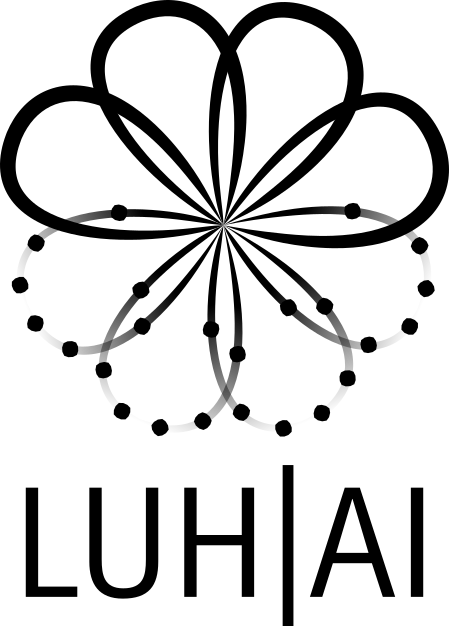
\includegraphics[height=\logoheight]{../latex_main/figures/logo_short}~
 
\includegraphics[height=\logoheight]{../latex_main/figures/luh_logo_rgb_0_80_155.pdf}
 	
	% 
\includegraphics[height=\logoheight]{figures/logo_tntluh.pdf}
}

% Header logo for title page
\settitleheaderimage{
	% 
\includegraphics[height=\logoheight]{figures/TNT_darkv4.pdf}
	
\includegraphics[height=\logoheight]{../latex_main/figures/luh_logo_rgb_0_80_155.pdf}
	% 
\includegraphics[height=\logoheight]{figures/logo_tntluh.pdf}
}

% Title page: tntdefault 
\setbeamertemplate{title page}[tntdefault]  % or luhstyle
% Add optional title image here
%\addtitlepageimagedefault{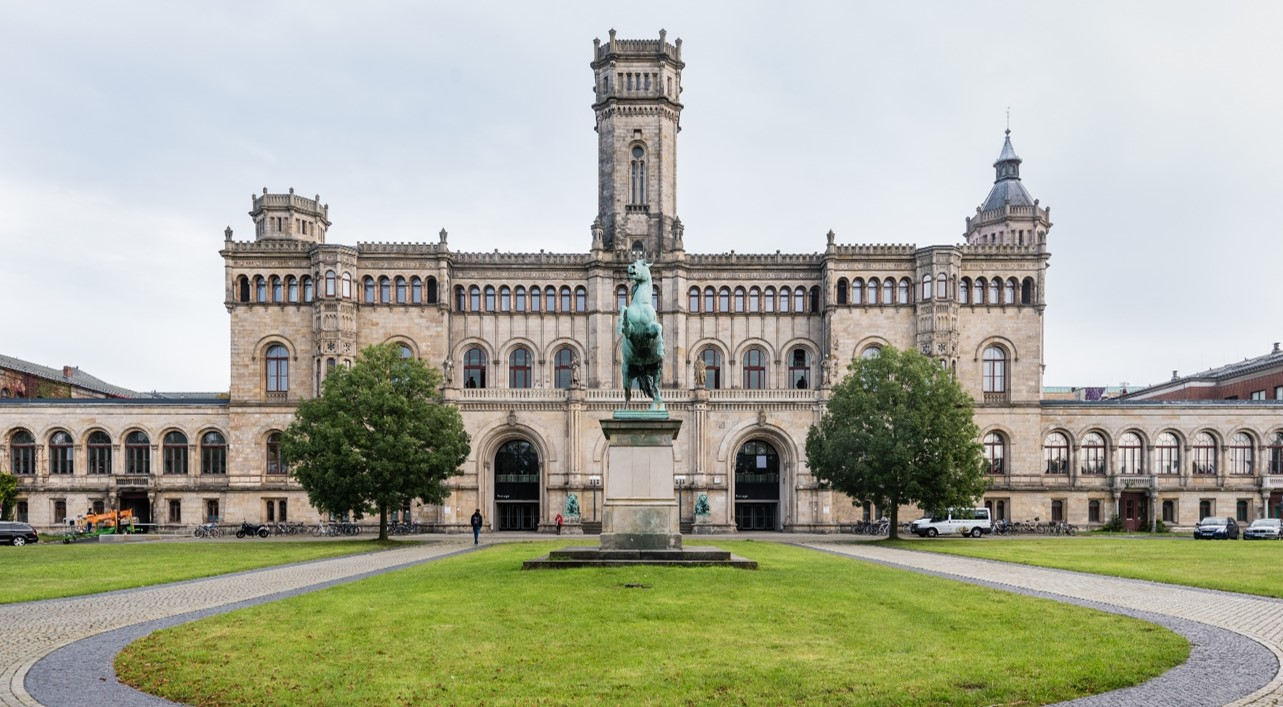
\includegraphics[width=0.65\textwidth]{figures/luh_default_presentation_title_image.jpg}}

% Title page: luhstyle
% \setbeamertemplate{title page}[luhstyle]
% % Add optional title image here
% \addtitlepageimage{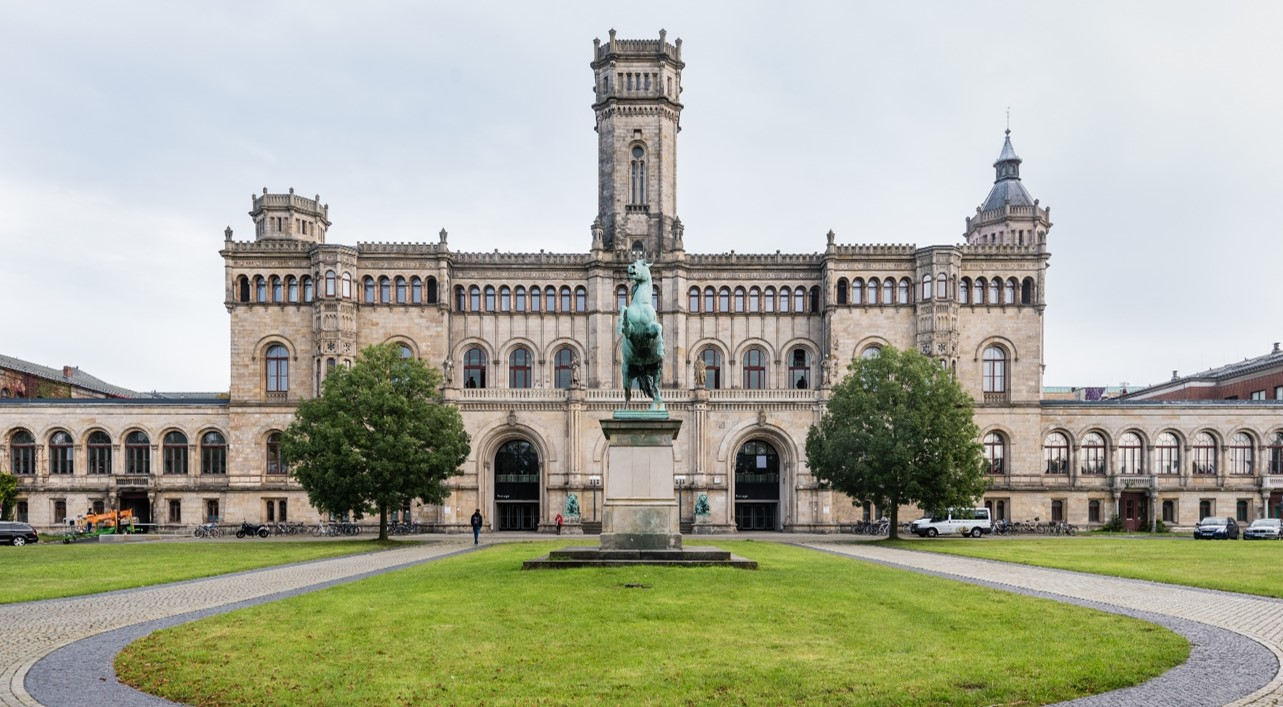
\includegraphics[width=0.75\textwidth]{figures/luh_default_presentation_title_image.jpg}}

\author[Marius Lindauer]{Marius Lindauer\\[1em]
	
\includegraphics[height=\logoheight]{../latex_main/figures/luh_logo_rgb_0_80_155.pdf}\qquad
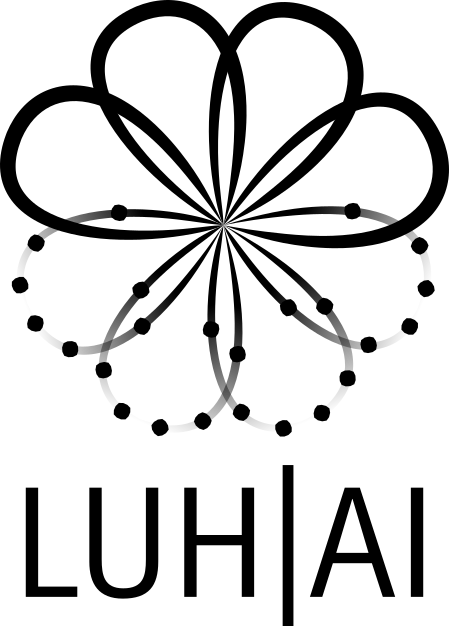
\includegraphics[height=2.2em]{../latex_main/figures/logo_short}\qquad
%
\includegraphics[height=2.2em]{../latex_main/figures/L3S.jpg}\qquad

\includegraphics[height=2.2em]{../latex_main/figures/LAA.png}}
\date{%Winter Term 2021/22
}


%%% Custom Packages
%----------------------------------------------------------------------
% Create dummy content
\usepackage{blindtext}

% Adds a frame with the current page layout. Just call \layout inside of a frame.
\usepackage{layout}

\title[RL: Policy Gradient]{RL: Policy Search}
\subtitle{Step Size and Trust Region}


\begin{document}
	
	\maketitle

%----------------------------------------------------------------------
%----------------------------------------------------------------------
\begin{frame}[c]{Policy Gradient and Step Size}
	
    \begin{itemize}
        \item Goal: Each step of policy gradient yields an updated policy $\pi'$ whose value is greater than (or equal) to the prior policy $\pi$: $V^{\pi'} \geq V^\pi$
        \begin{itemize}
            \item Monotonic improvement
            \item Important in some applications
            \item PG often more stable than DQN
        \end{itemize} 
        \item Gradient descent approaches update the weights a small step in direction of gradient
        \item First order / linear approximation of the value function's dependence on the policy parameterization
        \item Locally a good approximation; further aways less good
    \end{itemize}

\end{frame}
%-----------------------------------------------------------------------
%----------------------------------------------------------------------
\begin{frame}[c]{Why are step sizes a big deal in RL?}
	
    \begin{itemize}
        \item Step size is important in any problem involving the optima of a function
        \item Supervised learning: Step too far $\leadsto$ next updates might fix it
        \item Reinforcement learning:
        \begin{itemize}
            \item Step too far $\leadsto$ bad policy
            \item Next batch: collected under bad policy
            \item \alert{Policy is determining data collection!} 
            \begin{itemize}
                \item Essentially controlling exploration and exploitation trade-off due to particular policy parameters and the stochasticity of the policy
            \end{itemize}
            \item May not be able to recover from a bad choice $\leadsto$ collapse in performance
        \end{itemize}
    \end{itemize}

\end{frame}
%-----------------------------------------------------------------------
%----------------------------------------------------------------------
\begin{frame}[c]{Policy Gradient Methods with Auto-Step-Size Selection}
	
    \begin{itemize}
        \item Can we automatically ensure the updated policy $\pi'$ has value greater than (or equal to) the prior policy $V^{\pi'} \geq V^\pi$?
        \item Consider this for the policy gradient setting, and hope to address this by modifying step size
    \end{itemize}

\end{frame}
%-----------------------------------------------------------------------
%----------------------------------------------------------------------
\begin{frame}[c]{Objective Function}
	
    \begin{itemize}
        \item Goal: find policy parameters that maximize value function
        $$ V(\theta) = \mathbb{E}_{\pi_\theta} \left[ \sum_{t=0}^{\infty} \gamma^t r(s_t, a_t); \pi_\theta \right]$$
        \item have access to samples from the current policy $\pi_\theta$ 
        \item Want to predict the value of a different policy ($\leadsto$ off-policy learning)
    \end{itemize}

\end{frame}
%-----------------------------------------------------------------------
%----------------------------------------------------------------------
\begin{frame}[c]{Objective Function}
	\vspace{-1em}
    \begin{itemize}
        \item Goal: find policy parameters that maximize value function
        $$ V(\theta) = \mathbb{E}_{\pi_\theta} \left[ \sum_{t=0}^{\infty} \gamma^t r(s_t, a_t); \pi_\theta \right]$$
        \item Express value of $\Tilde{\pi}$ in terms of advantage of $\pi$
        \begin{eqnarray}
        V(\Tilde{\theta}) &=& V(\theta) + \mathbb{E}_{\pi{\Tilde{\theta}}} \left[ \sum_{t=0}^{\infty} \gamma^t A_\pi(s_t, a_t) \right]\\
        &=& V(\theta) + \sum_{s} \mu_{\Tilde{\pi}}(s) \sum_{a} \Tilde{\pi}(a \mid s) A_\pi(s_t, a_t) 
        \end{eqnarray}
        \item $ \mu_{\Tilde{\pi}}(s)$ is the discounted weighted frequency of state $s$ under policy $\Tilde{\pi}$
        \item We know the advantage $A_\pi$ and $\Tilde{\pi}$
        \item But we cannot compute the above we don't know $\mu(\Tilde{\pi})$, the state distribution under the newly proposed policy
    \end{itemize}

\end{frame}
%-----------------------------------------------------------------------
%----------------------------------------------------------------------
\begin{frame}[c]{Local Approximation}
	
    \begin{itemize}
        \item Can we remove the dependency on the discounted visitation frequencies under the new policy?
        \item Substitute in the discounted visitation frequency under the current policy to define a new objective function:
        $$ L_\pi(\Tilde{\pi}) = V(\theta) + \sum_{s} \alert{\mu_\pi (s)} + \sum_{a} \Tilde{\pi}(a \mid s) A_\pi(s,a)$$
        \item Note that $L_{\pi_{\theta_0}}(\pi_{\theta_0}) = V(\theta_0)$
        \item Gradient of $L$ is identical to gradient of value function at policy parameterized evaluated at $\theta_0$: 
        $$\nabla_{\theta} L_{\pi_{\theta_0}}(\pi_{\theta_0})\mid_{\theta = \theta_0} = \nabla_\theta V(\theta)\mid_{\theta = \theta_0}$$
    \end{itemize}

\end{frame}
%-----------------------------------------------------------------------
%----------------------------------------------------------------------
\begin{frame}[c]{Conservative Policy Iteration}
	
    \begin{itemize}
        \item Is there a bound on the performance of a new policy obtained by optimizing the surrogate objective?
        \item Consider mixture policies that blend an old policy and a different policy
        $$\pi_{new}(a \mid s) = (1 - \alpha) \pi_{old} (a \mid s) + \alpha \pi'(a \mid s) $$
        \item In this case, we can guarantee a lower bound on value of the new $\pi_{new}$:
        $$V^{\pi_{new}} \geq L_{\pi_{old}} (\pi_{new}) - \frac{2\epsilon\gamma}{(1- \gamma)^2} \alpha^2 $$
        where $\epsilon = \max_{s} \mathbb{E}_{a \sim \pi'(a \mid s) [A_\pi(s,a)]}$
    \end{itemize}

\end{frame}
%-----------------------------------------------------------------------
%----------------------------------------------------------------------
\begin{frame}[c]{Find the Lower-Bound in General Stochastic Policies}
	
	 \vspace{-1.5em}
    \begin{itemize}
        \item Would like to similarly obtain a lower bound on the potential performance for general stochastic policies (not just mixture policies)
        \item Recall $ L_\pi(\Tilde{\pi}) = V(\theta) + \sum_{s} \alert{\mu_\pi (s)} + \sum_{a} \Tilde{\pi}(a \mid s) A_\pi(s,a)$ 
    \end{itemize}
    
    \begin{block}{Theorem}
    Let $D_{TV}^{\max} (\pi_1, \pi_2) = \max_{s} D_{TV}(\pi_1(\cdot \mid s), \pi_2(\cdot\mid s)) = \max_{s} \max_{a} (\pi_1(a\mid s) -\pi_2 (a\mid s))$. Then
    $$V^{\pi_{new}} \geq L_{\pi_{old}} (\pi_{new}) - \frac{4\epsilon\gamma}{(1-\gamma)^2} (D_{TV}^{\max}(\pi_{old}, \pi_{new}))^2$$
    where $\epsilon = \max_{s,a}|A_\pi(s,a)|$
    \end{block}
    
    \begin{itemize}
        \item Note that $D_{TV}(p,q)^2 \leq D_{KL}(p,q)$ for prob. distribution $p$ and $q$
        \item Then the above theorem immediately implies that
        $$ V^{\pi_{new}} \geq  L_{\pi_{old}} (\pi_{new}) -  \frac{4\epsilon\gamma}{(1-\gamma)^2} D_{KL}^{\max}(\pi_{old}, \pi_{new}) $$
    \end{itemize}

\end{frame}
%-----------------------------------------------------------------------
%----------------------------------------------------------------------
\begin{frame}[c]{Optimization of Parameterized Policies}
	
    \begin{itemize}
        \item Goal is to optimize
        $$\max_{\theta}  L_{\pi_{old}} (\pi_{new}) -  \frac{4\epsilon\gamma}{(1-\gamma)^2} D_{KL}^{\max}(\pi_{old}, \pi_{new}) = L_{\pi_{old}} (\pi_{new}) -  C \cdot D_{KL}^{\max}(\pi_{old}, \pi_{new}) $$
        where $C$ is the penalty coefficient (i.e. hyperparameter)
        \item The penalty (from theory) would be fairly small in practice
        \medskip
        \item New Idea: Use a trust region constraint on step sizes. Do this by imposing a constraint on the KL divergence between the new and old policy:
        \begin{eqnarray}
        \max_{\theta} L_{\theta_{old}} (\theta)\\
        \text{subject to } D_{KL}^{s \sim \mu_{\theta_{old}}} (\theta_{old}, \theta) \leq \delta
        \end{eqnarray}
        \item This uses the average KL instead of max (the max requires the KL is bounded at all states and yields an impractical number of constraints)
    \end{itemize}
    
\end{frame}
%-----------------------------------------------------------------------
%----------------------------------------------------------------------
\begin{frame}[c]{From Theory to Practice}
	
    \begin{itemize}
        \item Prior objective:
        $$ \max_{\theta} L_{\theta_{old}} (\theta)$$
        {\centering subject to $ D_{KL}^{s \sim \alert{\mu_{\theta_{old}}}} (\theta_{old}, \theta) \leq \delta$\\}
        where $ L_\pi(\Tilde{\pi}) = V(\theta) + \sum_{s} \alert{\mu_\pi (s)} + \sum_{a} \Tilde{\pi}(a \mid s) \alert{A_\pi(s,a)}$ 
        \item Don't know the visitation weights nor true advantage function
        \pause
        \item Instead do the following substitutions:
        $$ \sum_{s} \mu_\pi (s) \to \frac{1}{1- \gamma} \mathbb{E}_{s\sim \mu_{\theta_{old}}} [\ldots]$$
        \item[$\leadsto$] estimate $\mu_\pi (s)$ wrt the sampled trajectories we have already
    \end{itemize}

\end{frame}
%-----------------------------------------------------------------------
%----------------------------------------------------------------------
\begin{frame}[c]{From Theory to Practice II}
	
    \begin{itemize}
        \item Next substitution:
        $$\sum_{a} \pi_\theta (a\mid s_n) A_{\theta_{old}} (s_n, a) \to \mathbb{E}\left[ \frac{\pi_\theta(a \mid s_n)}{q(a\mid s_n)} A_{\theta_{old}} (s_n, a) \right] $$
        \item where $q$ is some sampling distribution over actions and $s_n$ is a particular sampled state
        \item This second substitution is to use importance sampling to estimate the desired sum, enabling the use of an alternate sampling distribution $q$ (other than the new policy $\pi_\theta$)
        \pause
        \item Third substitution:
        $$ A_{\theta_{old}} \to Q_{\theta_{old}}$$
        \item Note that the above substitutions do not change the solution to the above optimization problem
    \end{itemize}

\end{frame}
%-----------------------------------------------------------------------
%----------------------------------------------------------------------
\begin{frame}[c]{Selecting the Sampling Policy}
	
    \begin{itemize}
        \item Optimize
        $$ \max_\theta \mathbb{E}_{s\sim \mu_{\theta_{old}}, a \sim q} \left[ \frac{\pi_\theta(a \mid s_n)}{q(a\mid s_n)} A_{\theta_{old}} (s_n, a) \right]$$
        {\centering subject to $\mathbb{E}_{s\sim \mu_{\theta_{old}}} D_{KL}(\pi_{old}(\cdot \mid s), \pi_\theta (\cdot \mid s)) \leq \delta$ \\}
        \item Standard approach: sampling distribution is $q(a\mid s)$ is simply $\pi_{old}(a \mid s)$
        \item For the vine procedure see the paper
    \end{itemize}
    
    \centering
    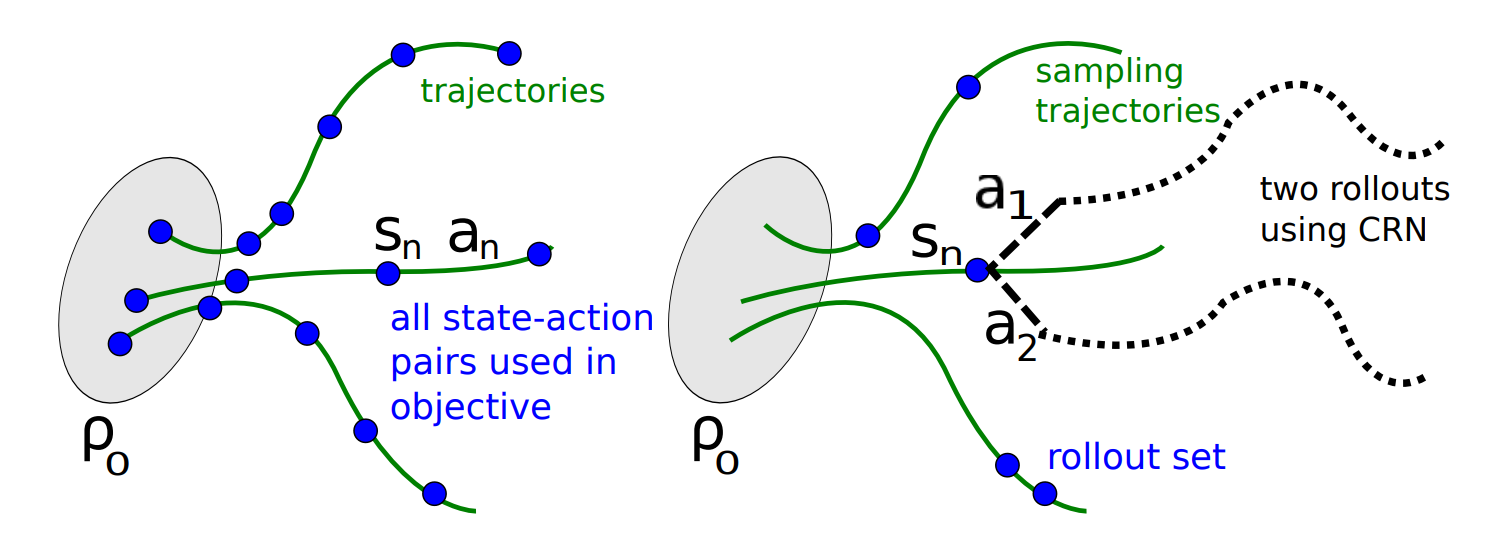
\includegraphics[width=0.5\textwidth]{w07_policy_search/images/trpo.PNG}\\
    \lit{Schulman et al. 2015}{https://arxiv.org/abs/1502.05477}

\end{frame}
%-----------------------------------------------------------------------
%----------------------------------------------------------------------
\begin{frame}[c]{TRPO Algorithm~\lit{Schulman et al. 2015}{https://arxiv.org/abs/1502.05477}}

	\begin{itemize}
	    \item For $i= 1,2,\ldots$ do
	    \begin{enumerate}
	        \item Run policy for $T$ timesteps or $N$ trajectories
	        \item Estimate advantage function at all timesteps
	        \item Compute estimated policy gradient $\hat{g}$
	        \item Use CG to compute $F^{-1}g$ where F is the fisher information matrix
	        \item Do line search on surrogate loss $L$ and KL constraint
	    \end{enumerate}
	\end{itemize}



\end{frame}
%-----------------------------------------------------------------------
%----------------------------------------------------------------------
\begin{frame}[c]{Common Template of Policy Gradient Algorithms}

	\begin{itemize}
	    \item For $i= 1,2,\ldots$ do
	    \begin{enumerate}
	        \item Run policy for $T$ timesteps or $N$ trajectories
	        \item At each timestep in each trajectory, compute target $Q^\pi(s_t, a_t)$ and baseline $b(s_t)$
	        \item Compute estimated policy gradient $\hat{g}$
	        \item Update the policy using $\hat{g}$, potentially constrained to a local region (i.e., try to ensure monotonic improviement)
	    \end{enumerate}
	\end{itemize}



\end{frame}
%-----------------------------------------------------------------------
%----------------------------------------------------------------------
\begin{frame}[c]{Policy Gradient Summary}

\begin{itemize}
    \item Extremely popular and useful set of approaches
    \item Can input prior knowledge in the form of specifying policy parameterization
    \item You should be familiar with REINFORCE and the policy gradient template on the previous slide
    \item Understand the where different estimators can be slotted in 
    \item Don't have to be able to derive or remember the specific formulars in TRPO for approximating the objectives and constraints
\end{itemize}

\end{frame}
%-----------------------------------------------------------------------
%-----------------------------------------------------------------------
\end{document}
